\chapter*{\LARGE Appendices}


\addcontentsline{toc}{chapter}{Appendices}
% Temporarily adjust tocdepth so sections do not appear in the main TOC
\addtocontents{toc}{\protect\setcounter{tocdepth}{-1}}
\renewcommand{\thesection}{\Alph{section}}
\adjustmtc 
% mini table of contents for appendices
\minitoc
% Restore normal tocdepth for sections within the appendices
\setcounter{tocdepth}{2}

%%%%%%%%%%%%%%%%%%%%%%%%%%%%%%%%%%%%%%%%%%%%%%%%%%
%%%%%%%%%%%%%%%%%%%%%%%%%%%%%%%%%%%%%%%%%%%%%%%%%%
\section{Data descriptions and variable creation details}
%%%%%%%%%%%%%%%%%%%%%%%%%%%%%%%%%%%%%%%%%%%%%%%%%%
%%%%%%%%%%%%%%%%%%%%%%%%%%%%%%%%%%%%%%%%%%%%%%%%%%


This section details how the data used in this paper was collected and processed. I describe in turn the data sources mentioned in Table \ref{tab:data_sources}. The codebook (Table \ref{tab:codebook}) serves as further reference.

%%%%%%%%%%%%%%%%%%%%%%%%%%%%%%%%%%
\subsection{GASPAR Database}

In the raw GASPAR database, each row corresponds to a single hazard clause of a natural catastrophe decree published in the \textit{Journal Officiel}—that is, one commune, one hazard, and one time window. Each decree is identified by a unique code CatNat, but when multiple hazards are recognized within the same decree (e.g. both flooding and landslides), the identifier is repeated, generating one row per hazard. As a result, raw counts of code CatNat overstate the number of distinct events. To avoid this double-counting, I collapse the data to the commune × hazard × calendar-year level, treating all rows that share these three keys as a single disaster episode within a commune. The resulting event counts are reported in Table \ref{tab:flood_summary}. Figure \ref{fig:durat_categories} plots the distribution of durations for all recorded flood events, which serves as the basis for defining my three categories of flood intensity. \\
%It would be interesting to plot here trend in GASPAR CatNat and Floods CatNats, disuss how this could be biased. i alrady did that graph.


  \begin{figure}[htbp]
    \centering
    \caption{\textbf{Figure \ref{fig:durat_categories}:}  Distribution of flood event durations}
    \label{fig:durat_categories}
    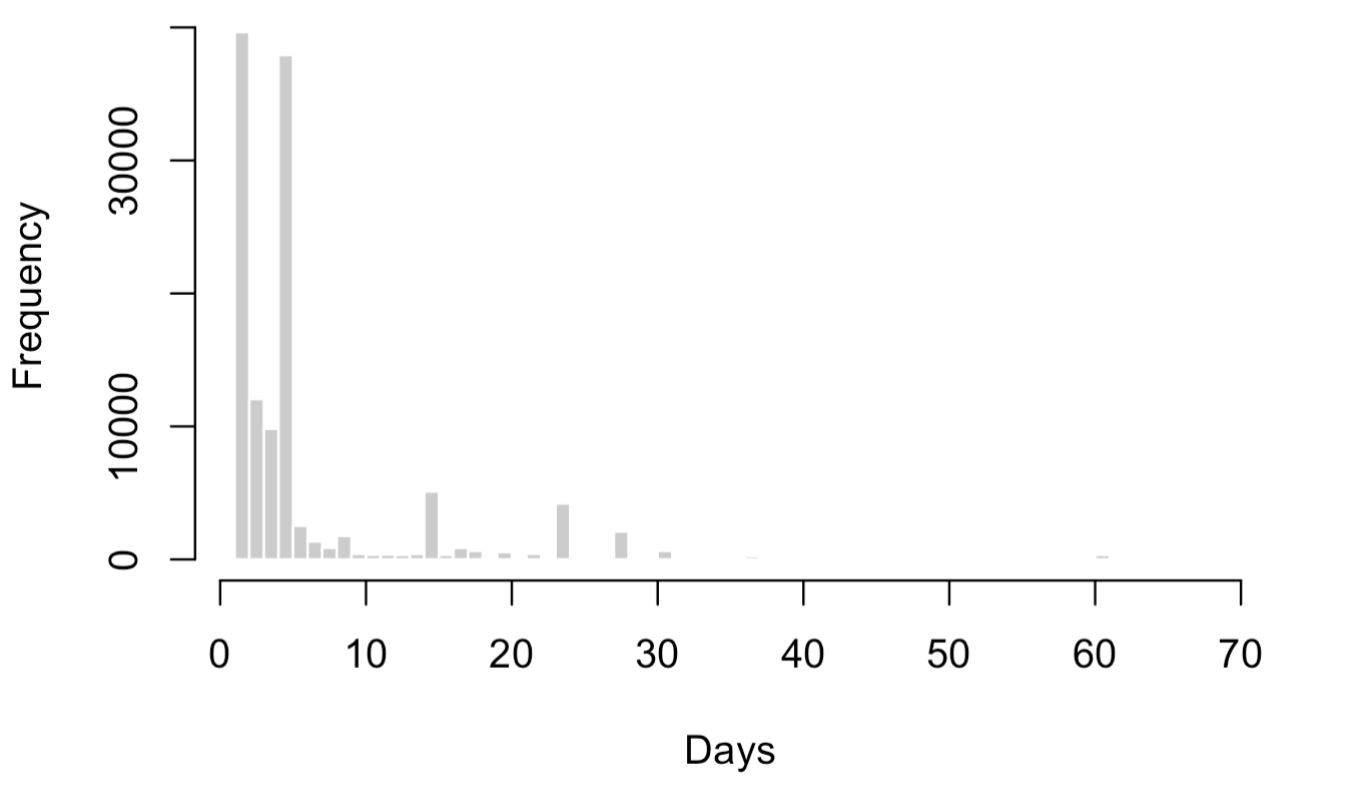
\includegraphics[width=0.9\textwidth]{figures/Data/duration_flood_gaspar.png}

    %\caption*{\raggedright\textit{Note}:}
    
    \end{figure}


%%%%%%%%%%%%%%%%%%%%%%%%%%%%%%%%%%%
\subsection{Long Term Flood Exposure Index}
\label{ch:appendix_risk_index}


\noindent
Utilizing high‐resolution floodplain maps of Europe provided by \citet{dottori_et_al_2022}, I propose and develop a time-invariant flood risk index that is used to stratify the econometric analysis and guide sample selections. I choose the floodplain map with RP100 floods, indicating the extent of flooding that is statistically expected to be equaled or exceeded on average once every 100 years, a standard return period used in insurance and urban planning. I overlay the RP100 raster (GeoTIFF) data—a grid of 90m × 90m cells, each with a continuous value of water depth (in meters)—onto the polygons of all communes in metropolitan France. Counting how many of the raster cells fall within the boundaries of a commune, and then converting cell counts to surface areas, allows me to compute the percentage share of a commune's total area that is exposed to varying intensities of flood risk. Following categorization schemes used by the European Commission’s \href{https://drmkc.jrc.ec.europa.eu/risk-data-hub#/}{Risk
 Data Hub} and in the PESETA reports, I classify exposure intensity of each raster cell into four bands: $(0–0.5m]$, $(0.5–1.5m]$, $(1.5–3m]$, and $>3m$. The distribution of water depth values is heavily right-skewed, as shown in Figure \ref{fig:raster_values_distrib}. For each commune, the risk index is simply built as the sum of four variables, capturing the proportion of the commune’s total surface falling into each of the four depth bands, and excluding “unflooded” remainder. The risk index thus ranges from 0 to 100, and is plotted in Figure \ref{fig:risk_index}; it can be conceived as the share of each commune’s surface that is colored in purple in Figure \ref{fig:raster_unbinned}. Several flood risk or exposure indices are used in the academic literature—alongside \cite{indaco2024adapting} and \cite{hussain2024flooding}. Other indices range from global event-based \citep{okazawa2011development}, local exposure-vulnerability \cite{anindita2020flood}, GIS susceptibility models, to composite social-exposure indices and macro-scale global indices (WorldRiskIndex). These indices go in the direction of the damage function in \cite{carleton2022valuing} and, more specifically for our application, the damage functions in \cite{bilal2023anticipating}.

This measure of flood hazard could be refined in several ways. Rather than relying on a simple sum of flooded area across intensity categories, a weighted sum—placing greater emphasis on more severe flooding—would better reflect the nonlinear relationship between water depth and economic damage often observed in engineering and insurance data \cite{ballocci2024econometric}. For example, a commune that is 30\% flooded at 2 meters likely faces far greater losses than one that is 100\% flooded at 5 cm. Similarly, exploiting multiple return periods (e.g., RP10 vs. RP500) would allow the index to capture temporal variation in exposure, distinguishing between persistently exposed areas and those facing latent, tail risks. These “risk-jumpers” can be identified by subtracting RP10 from RP500 flood depths—a difference that preliminary analysis has shown to be minimal in most regions but notable in places like the Loire Valley around the city of Orléans, highlighting the importance of such hazard maps in informing investments in resilience across France. As explained in Section \ref{ch: discussion}, to improve precision of my estimates, beyond the risk index I include other time-invariant covariates in my specification, such as the share of establishments covered by EAIP (Figure \ref{fig:eaip_map}) and commune median revenue. I also test other covariates that could have been included directly in the index. Table \ref{tab:pscore_logit} shows results.

%Table X reports the share of communes classified as “risk-jumpers” (large RP500 vs. RP10 exposure) by region versus those under chronic risk, as well as other statistics around the risk index (including correlation with CatNat events). 

Finally, in integrated structural models of climate change, a flood risk index at the commune level could act as an amenity shifter that affects the relative desirability of locations. Households and firms are assumed to sort spatially based on wages, prices, and local amenities, influencing spatial sorting and long-run equilibrium under evolving climate risk. By simulating these equilibria under different flood scenarios (e.g., comparing RP10 vs. RP500), the model can generate forward-looking predictions of where people and firms are likely to concentrate or retreat. %offering a powerful tool for long-term planning and adaptation policy.
\vspace{0.3cm}

\begin{figure}[!htbp]

  \centering
  % first subfigure at 49% of text width
  \caption{\textbf{Figure \ref{fig:raster_flood}:} Hazard exposure - Flood raster data (RP100)}
  \label{fig:raster_flood}
  \begin{subfigure}[b]{0.44\textwidth}
    \centering
    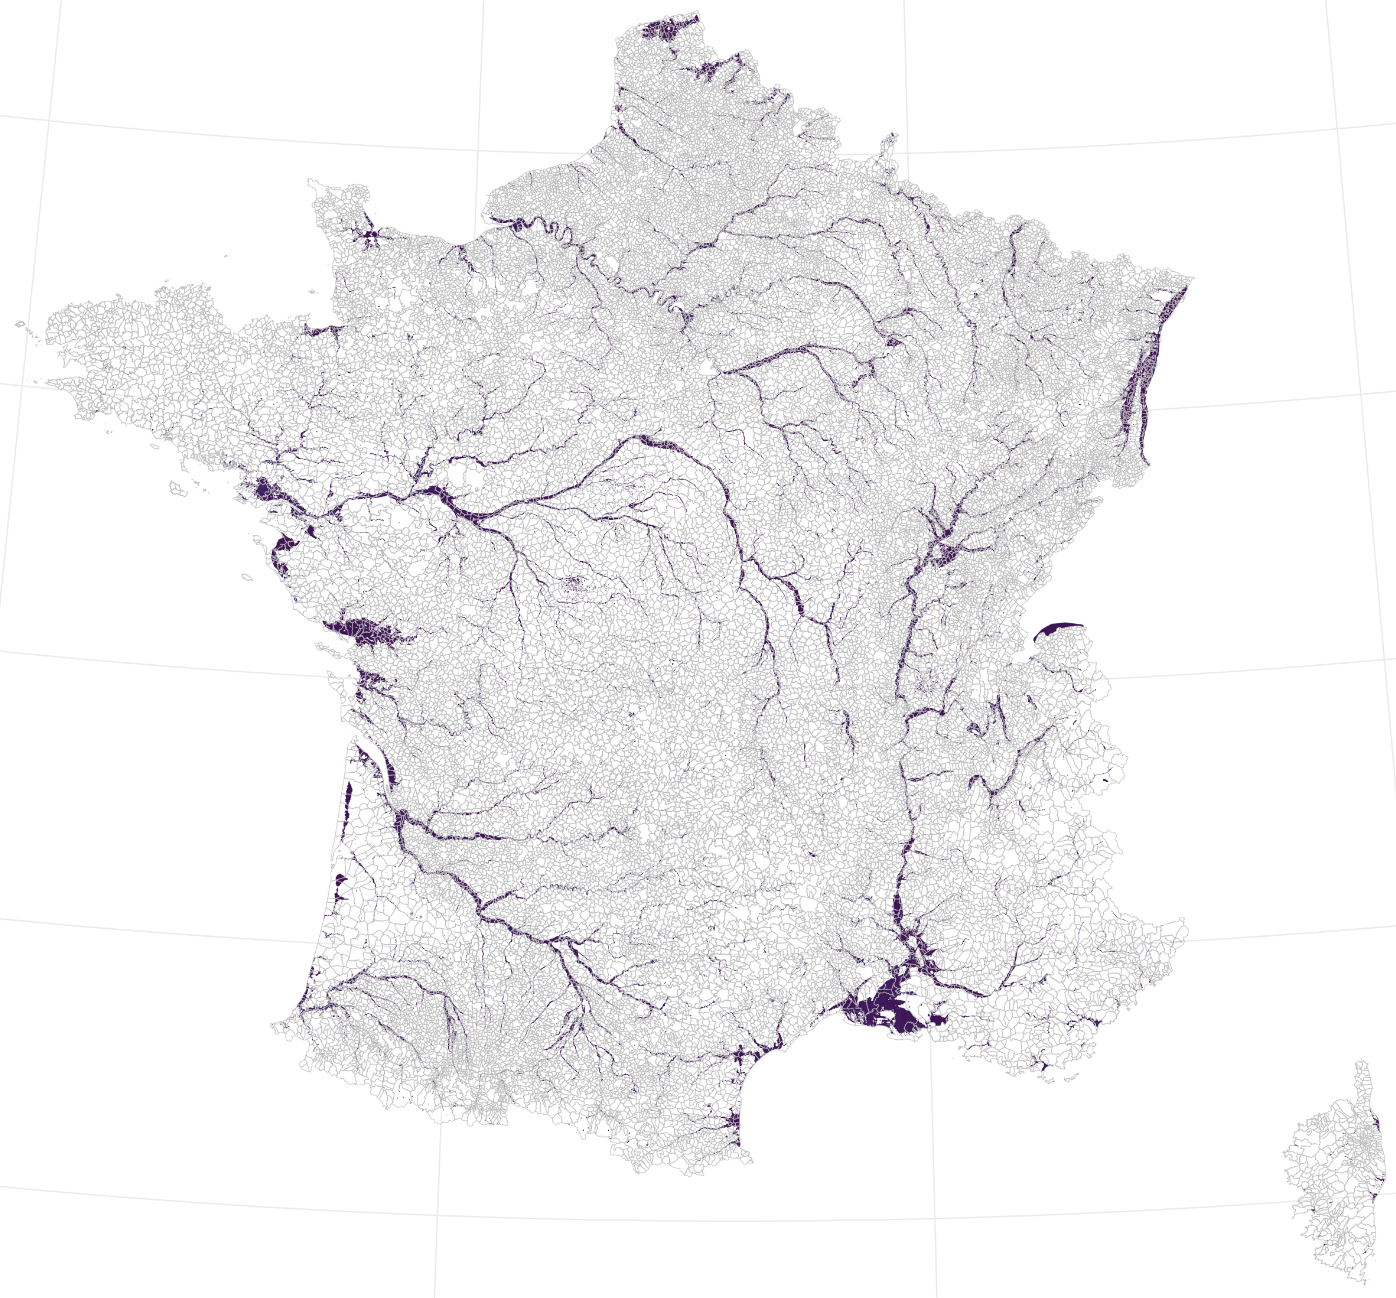
\includegraphics[width=\linewidth]{figures/Data/Raster Unbinned.png}
    \subcaption{Extensive margin of ex-ante risk}
    \label{fig:raster_unbinned}
  \end{subfigure}%i
  % tiny horizontal skip, then second
  \hspace{0.02\textwidth}%
  \begin{subfigure}[b]{0.536\textwidth}
    \centering
    
\includegraphics[width=\linewidth]{figures/Data/Raster Binned.png}
    \subcaption{Intensive margin of ex-ante risk}
    \label{fig:raster_binned}
\end{subfigure}



\end{figure}


\begin{figure}[!htbp]
    \centering
    \caption{\textbf{Figure \ref{fig:raster_values_distrib}:} Histogram of RP100 flood‐depth values at 90m×90m resolution}
    \label{fig:raster_values_distrib}
    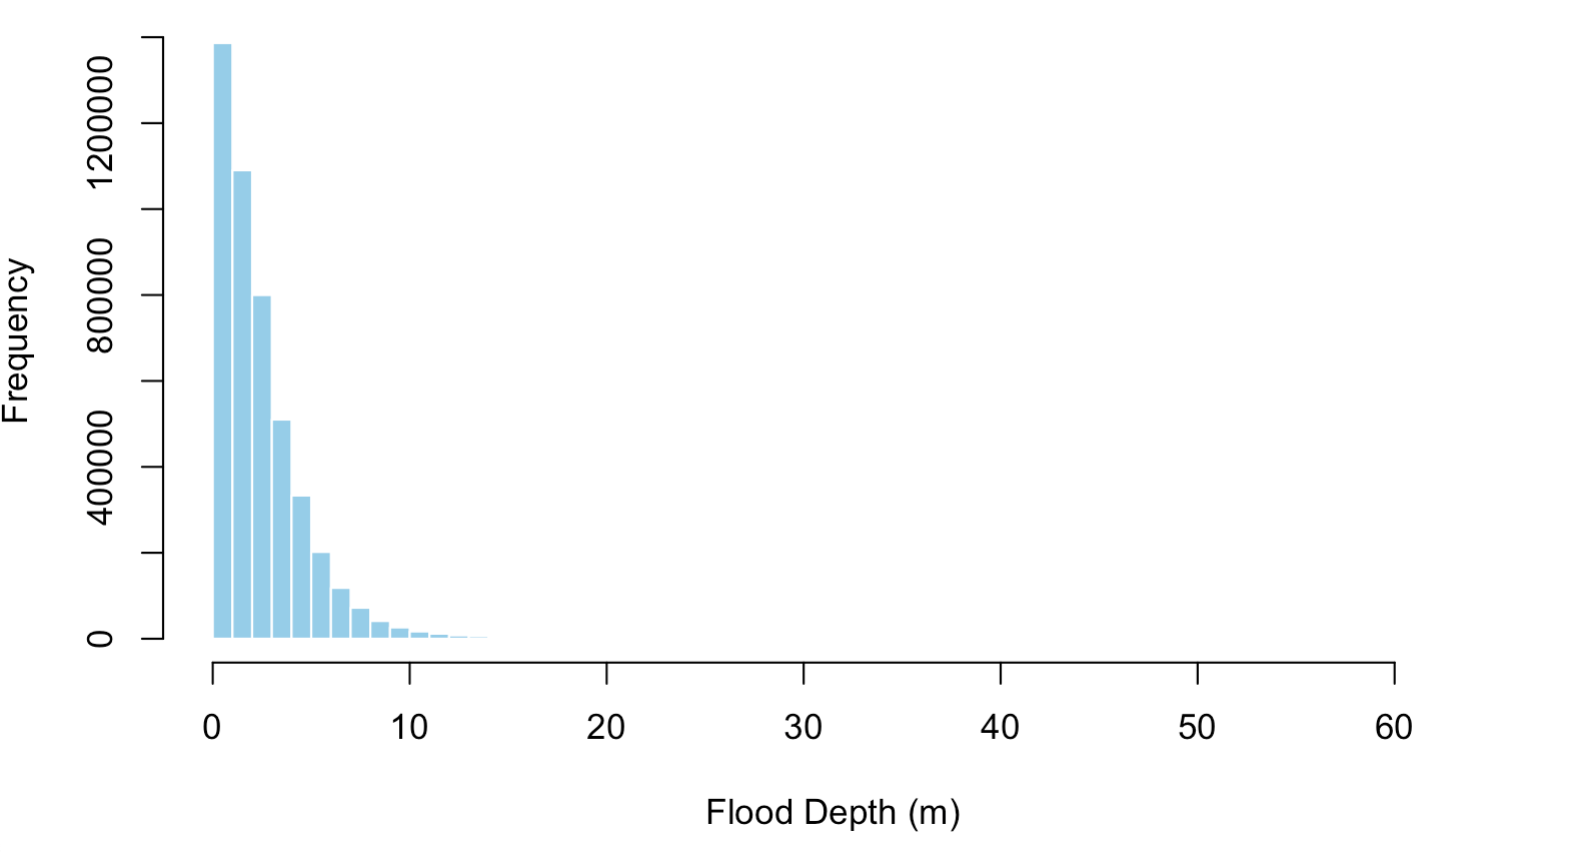
\includegraphics[width=0.7\textwidth]{figures/Data/Raster depth values.png}
    \caption*{\raggedright\textit{Note}: The distribution is markedly right-skewed: the vast majority of pixels record minimal inundation, while a small tail captures the comparatively rare, deeper flood depths. Furthermore, 90\% of all flooded cells fall between 0.07 and 3 meters in water depth.}
    
    \end{figure}


\begin{figure}[!htbp]
    \centering
    \caption{\textbf{Figure \ref{fig:risk_disribu}:} Histogram of Flood Risk Index values at commune level}
    \label{fig:risk_disribu}
    
    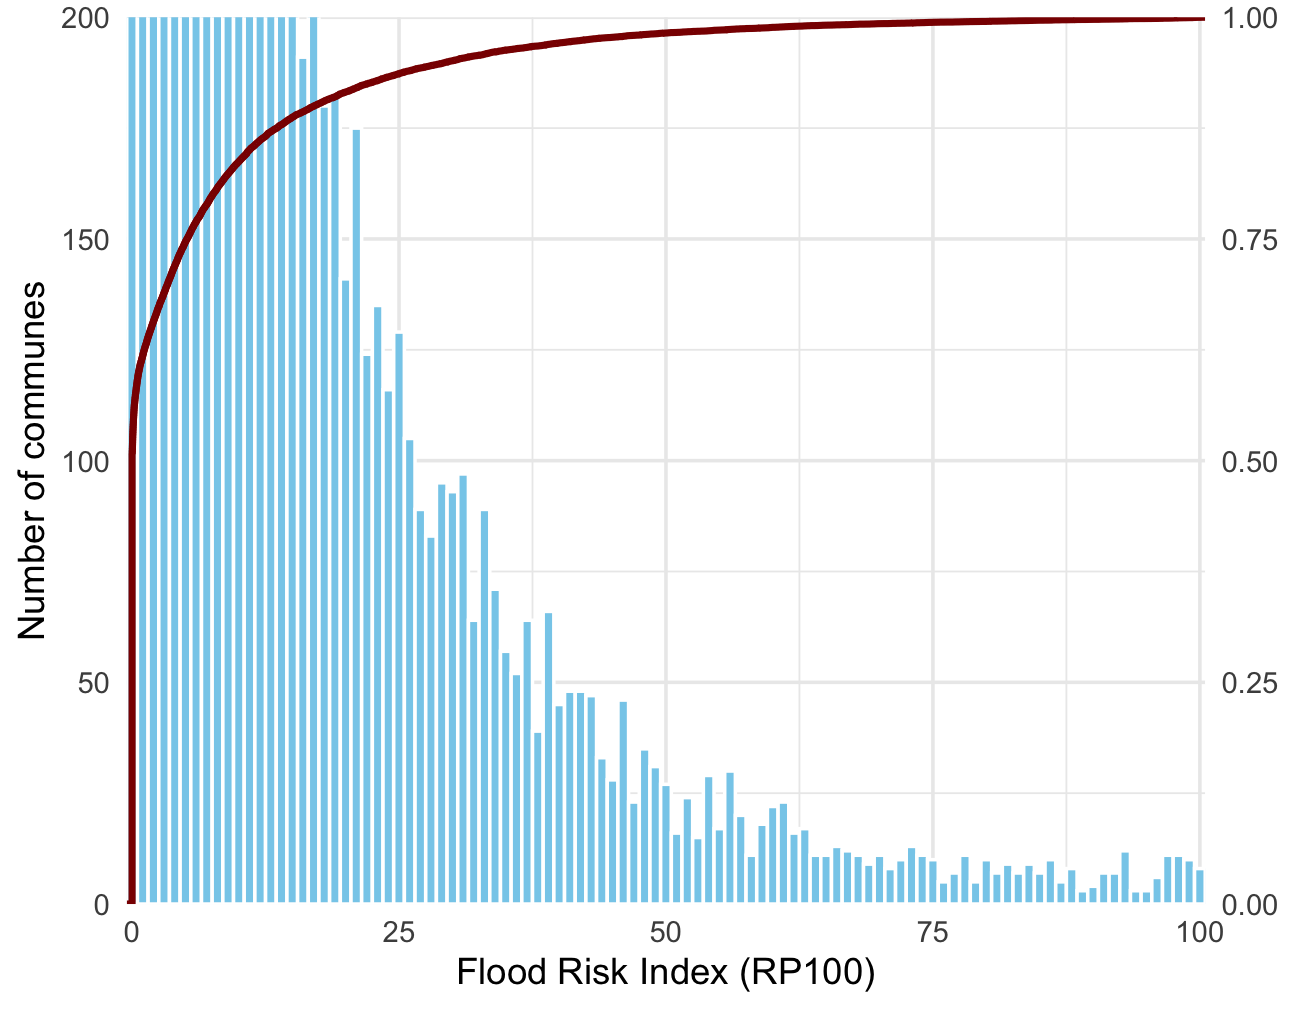
\includegraphics[width=0.7\textwidth]{figures/Data/disribution risk index.png}
    %\caption*{\raggedright\textit{Note: The distribution of the index}}
    
    \end{figure}













%%%%%%%%%%%%%%%%%%%%%%%%%%%%%%%%%

\subsection{Propensity Score}
\label{ch:pscore_appendix}
To improve covariate balance between treated and control firms, and hence precision, I estimate a propensity score for flood exposure using pre-determined firm and location characteristics, following a specification similar to \cite{fatica2024floods}.

As long as unconfoundedness is assumed and common support is established, IPW estimators can be used to estimate ATE and ATT effects. While ATE weights ask what would happen if a randomly selected firm were flooded, ATT weights estimate how floods affected firms that were actually flooded. Given my interest in realized flood shocks, I focus on the ATT. I examine the distribution of the propensity score across treatment status. I then use the score to construct analytical weights. The ATT weights are of the form:

\noindent\text{weights given by}
\begin{align*} w_1^{att}(D) &= \frac{D}{\mathbb{E}[D]}, \\ w_0^{att}(D, p(X)) &= \frac{\frac{(1 - D)p(X)}{1 - p(X)}}{\mathbb{E}\left[ \frac{(1 - D)p(X)}{1 - p(X)} \right]}. \end{align*}

I begin with a pooled logit that relies only on time-invariant firm characteristics, whose result is presented in Table \ref{tab:pscore_logit}. Once the propensity score is known, I build the ATT weights as described above and proceed with standard inference procedures, re-estimate the outcome model on this re-weighted sample. The distribution of $p(x)$ in the adjusted and unadjusted sample is shown in Figure \ref{fig:pscore_distr}, while Figure \ref{fig:ps_cov_balance} illustrates the improvement in covariate balance achieved by the computed weights.

\vspace{1cm}

\begin{table}[!htbp] 
\centering 
\caption{\textbf{Table \ref{tab:pscore_logit}:} \textsc{Propensity-score logit for extreme floods (2010–2019)}} 
\label{tab:pscore_logit}

 \resizebox{12cm}{!}{
\begin{tabular}{@{\extracolsep{6pt}}p{8cm} c} 
\\[-1.8ex]\hline 
\hline \\[-1.8ex] 
& \textit{Dependent variable:}\\ 
\cline{2-2} 
\\[-1.8ex] & Extreme-flood dummy\\ 
\hline \\[-1.8ex] 
Flood–risk-group decile            & 0.160$^{***}$ \\ 
                                   & (0.029)        \\[0.15em]

Share of establishments under EAIP & 0.219          \\ 
                                   & (0.280)        \\[0.15em]

Income category of commune         & 0.0334         \\ 
                                   & (0.088)        \\[0.15em]

Urban dummy                        & 0.456$^{***}$  \\ 
                                   & (0.073)        \\[0.15em]

Coastal dummy (littoral sea)       & 0.908$^{***}$  \\ 
                                   & (0.127)        \\[0.15em]

Floods 1982–1999 (count)           & $-$0.118$^{***}$ \\ 
                                   & (0.044)        \\[0.15em]

Constant                           & $-$3.476$^{***}$ \\ 
                                   & (0.206)        \\[0.35em]
\hline \\[-1.8ex] 
Observations                       & 6,676,631       \\ 
Wald $\chi^2$(6)                   & 178.33          \\ 
Pseudo R$^2$                       & 0.0293          \\ 
Log pseudolikelihood               & $-$1,564,659.3  \\ 
\hline 
\hline \\[-1.8ex] 
\multicolumn{2}{p{13cm}}{\textit{Note:} $^{*}p<$0.1; $^{**}p<$0.05; $^{***}p<$0.01. Robust standard errors clustered at the commune level. Coastal dummy includes only sea-type areas (89\% of cases). Interestingly, the coefficient for floods occurring in 1982–1999 is negative, possibly indicating that adaptation to flooding has taken place in communes more heavily exposed in the past, now resulting in fewer CatNat declarations.} \\ 
\end{tabular}}
\end{table}

% , the next steps are: 1) convert the obtained propensity scores to IPW (ATE) or ATT weights, then compute MSD in the IPW-weighted data so that treated and control groups share the same covariate distribution, and ; 2) apply doubly-robust IPW-RA; 3) nearest-neighbor matching, pairing each flooded commune with the dry commune that has the closest propensity score and computing the mean outcome gap within those matched pairs; 4) drop units whose predicted score is near 0 or 1, keeping only the range where both treated and control communes exist, then run the analysis on that trimmed sample.

% Since I cannot estimate ATE (there is selection into treatment), I estimate ATT effects. The weights are built as $\frac{e_i}{1-e_i}$ for controls. Balance is shown after matching.



% \noindent To capture common calendar-year shocks and unobserved heterogeneity across firms, one could also estimate a more nuanced model such as:

% \begin{equation}
% \Pr!\bigl(D_{it}=1 ,\big|, X_i, T_t, u_i\bigr)=
% \Phi!\Bigl(\alpha X_i+\delta T_t+u_i\Bigr)
% \end{equation}

% This would allow estimation of a more accurate propensity score.


\begin{figure}[htbp]
\centering
\caption{\textbf{Figure \ref{fig:ps_cov_balance}:} Covariate balance before and after matching}
\label{fig:ps_cov_balance}
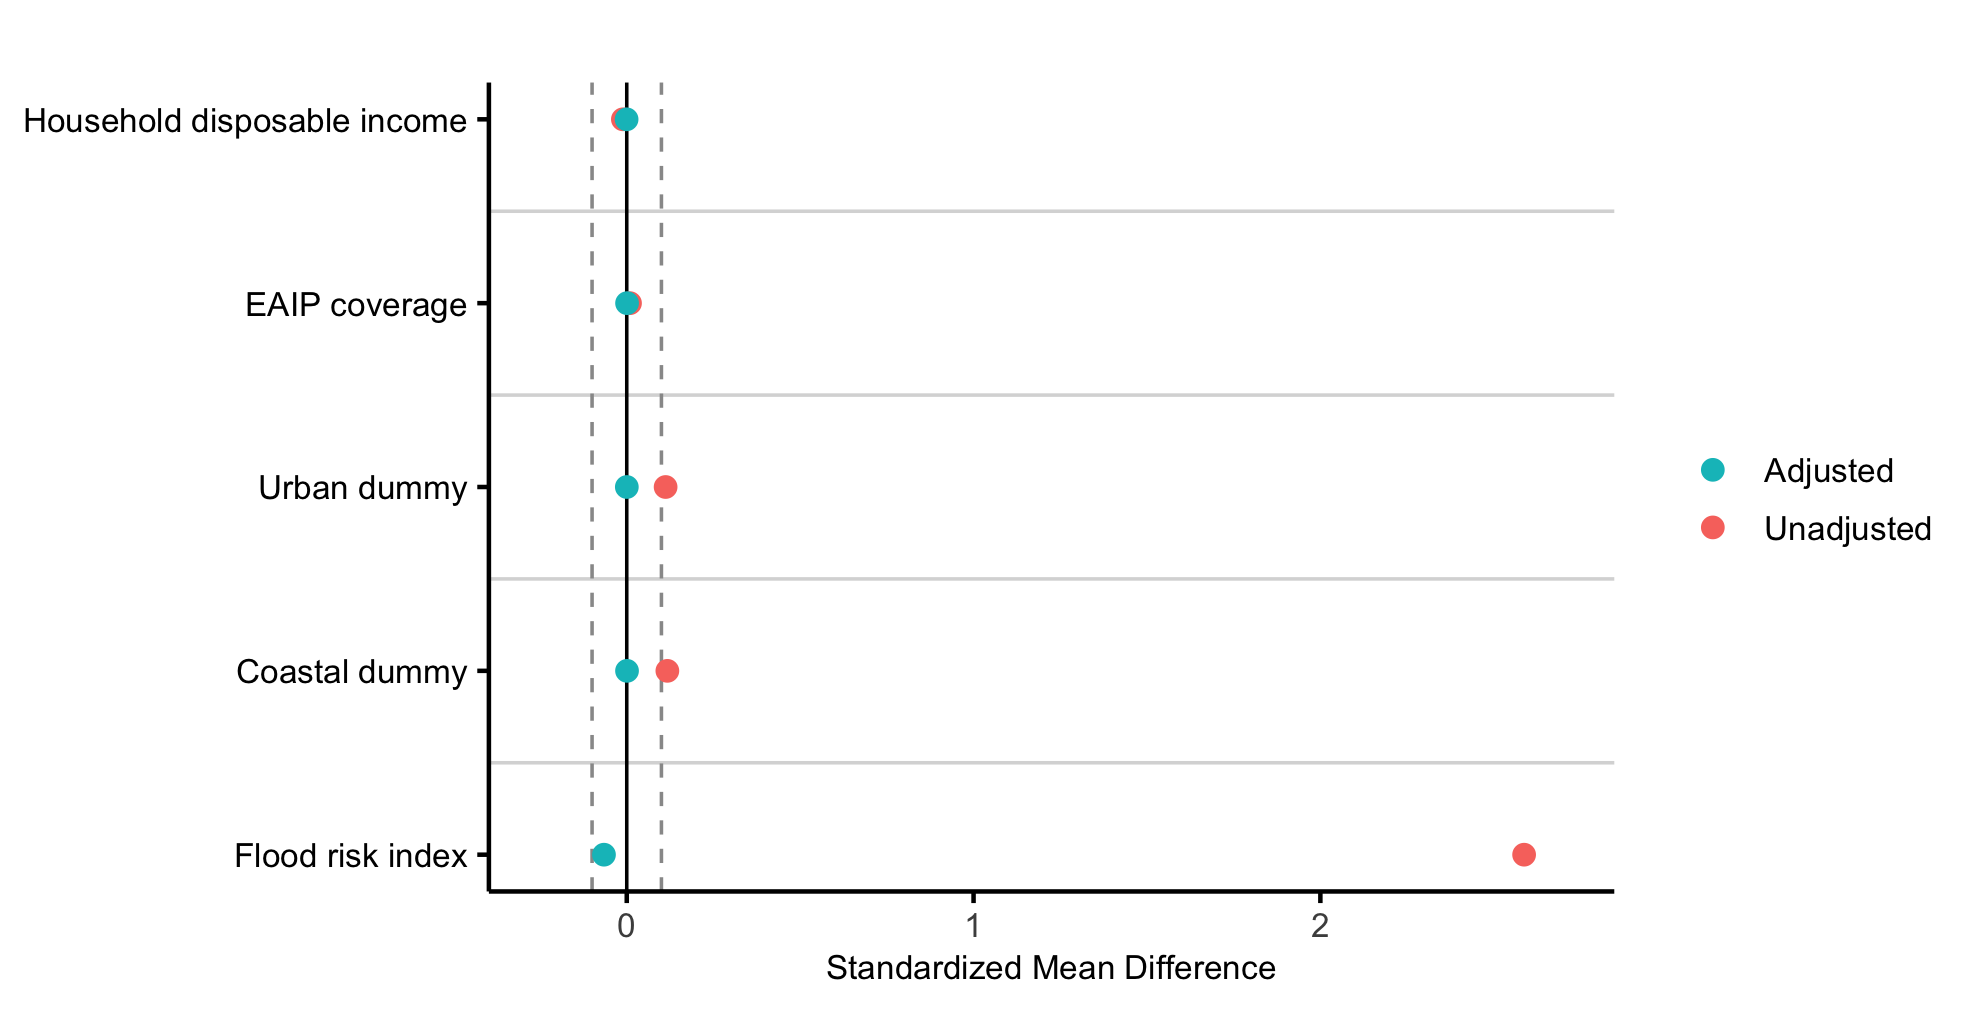
\includegraphics[width=0.86\textwidth]{figures/PScore/covariate_balance.png}
\caption*{\raggedright\textit{Note}: Flood risk index is an outlier with 2.59 SMD in the unadjusted sample.}
\end{figure}

\vspace{0.2cm}

\begin{figure}[htbp]
\centering
\caption{\textbf{Figure \ref{fig:pscore_distr}}: Propensity score distribution}
\label{fig:pscore_distr}
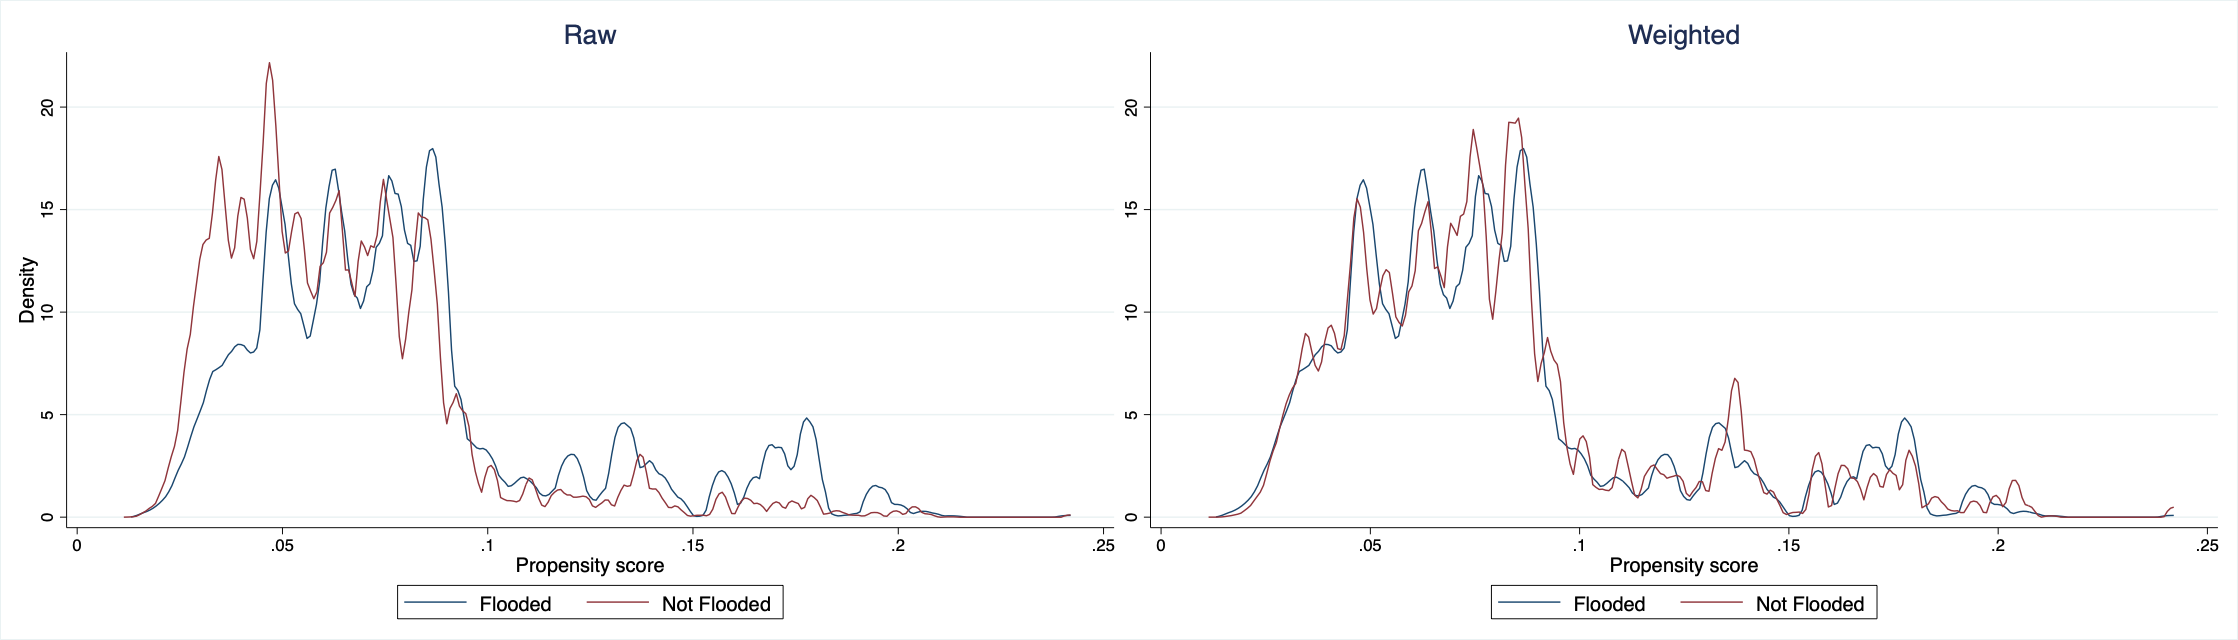
\includegraphics[width=1\textwidth]{figures/PScore/pscore_distrib.png}
\caption*{\raggedright\textit{Note}: The figure displays the distributions of the propensity scores before and after weighting, restricted to the region of common support. 2.12\% of the sample (N=144,299) is excluded because it is not in common support.}
\end{figure}


%%%%%%%%%%%%%%%%%%%%%%%%%%%%%%%%%%%%%%%%%%%%%%%%%%
%%%%%%%%%%%%%%%%%%%%%%%%%%%%%%%%%%%%%%%%%%%%%%%%%%
\clearpage
\section{Additional empirical results}
\label{sec:appendix_empirical}
%%%%%%%%%%%%%%%%%%%%%%%%%%%%%%%%%%%%%%%%%%%%%%%%%%
%%%%%%%%%%%%%%%%%%%%%%%%%%%%%%%%%%%%%%%%%%%%%%%%%%



\begin{table}[htbp]
\centering
\caption{\textbf{Table \ref{tab:stacked_es_employment_wages}:} \textsc{Stacked Event Study Estimates for Employment and Wages}}
\label{tab:stacked_es_employment_wages}


\resizebox{16cm}{!}{
\begin{tabular}{@{\extracolsep{6pt}}p{6.5cm}cccc}
\\[-1.8ex]\hline
\hline \\[-1.8ex]
& \multicolumn{4}{c}{\textit{Dependent variable:}} \\
\cline{2-5}
\\[-1.8ex] 
& \multicolumn{2}{c}{Headcount 31.12} & \multicolumn{2}{c}{Average wage at 31.12} \\
& (1) & (2) & (1) & (2) \\
\hline \\[-1.8ex]
\textbf{A. Post-Treatment Average Effect} \\[0.15em]
Treated $\times$ Post & $-$0.071 & $-$0.150$^{**}$ & $-$135.01$^{***}$ & $-$233.62$^{***}$ \\
                            & (0.045)  & (0.063)         & (41.98)           & (77.57)           \\[0.3em]

\textbf{B. Event-Study Estimates} \\[0.15em]
Treated $\times$ Event-time, $-5$ & $-$0.028 & $-$0.031 & $-$48.52 & $-$16.83 \\
                                 & (0.021)  & (0.033)  & (31.91)  & (48.47)  \\[0.15em]
Treated $\times$ Event-time, $-4$ & 0.008    & 0.027    & $-$52.54$^{**}$ & $-$40.41 \\
                                 & (0.015)  & (0.027)  & (26.37)  & (42.21)  \\[0.15em]
Treated $\times$ Event-time, $-3$ & $-$0.013 & 0.015    & 17.24    & $-$33.38 \\
                                 & (0.014)  & (0.019)  & (25.30)  & (37.73)  \\[0.15em]
Treated $\times$ Event-time, $-2$ & $-$0.013 & $-$0.004 & $-$2.72  & $-$45.89 \\
                                 & (0.013)  & (0.016)  & (25.38)  & (37.39)  \\[0.15em]
Treated $\times$ Event-time, $\phantom{-} 0$  & $-$0.083$^{***}$ & $-$0.169$^{***}$ & $-$186.67$^{***}$ & $-$214.19$^{***}$ \\
                                 & (0.020)         & (0.040)         & (19.88)         & (30.07) \\[0.15em]
Treated $\times$ Event-time, $+1$ & $-$0.114$^{***}$ & $-$0.230$^{***}$ & $-$122.83$^{***}$ & $-$268.61$^{***}$ \\
                                 & (0.036)         & (0.055)         & (27.40)         & (49.05) \\[0.15em]
Treated $\times$ Event-time, $+2$ & $-$0.057$^{*}$   & $-$0.088$^{*}$   & $-$186.74$^{***}$ & $-$236.09$^{***}$ \\
                                 & (0.029)         & (0.045)         & (27.62)         & (62.64) \\[0.15em]
Treated $\times$ Event-time, $+3$ & $-$0.216$^{***}$ & $-$0.144$^{***}$ & $-$165.92$^{***}$ & $-$185.56$^{***}$ \\
                                 & (0.042)         & (0.055)         & (31.77)         & (65.99) \\[0.15em]
Treated $\times$ Event-time, $+4$ & $-$0.132$^{***}$ & $-$0.163$^{***}$ & $-$180.45$^{***}$ & $-$202.26$^{***}$ \\
                                 & (0.034)         & (0.056)         & (38.06)         & (69.77) \\[0.15em]
Treated $\times$ Event-time, $+5$ & $-$0.124$^{**}$  & $-$0.176$^{**}$  & $-$84.79$^{*}$    & $-$187.39$^{**}$  \\
                                 & (0.056)         & (0.082)         & (47.21)         & (80.31) \\[0.35em]


\hline \\[-1.8ex]
Total observations                & 6.82M & 6.82M & 6.82M & 6.82M \\
Variance weighted (stacked) weights               & Yes    & Yes   & Yes    & Yes   \\
ATT weights               & No    & Yes   & No    & Yes   \\
Fixed effects               & Yes   & Yes   & Yes   & Yes   \\
\hline
\hline \\[-1.8ex]
\multicolumn{5}{p{17cm}}{\textit{Note:} Model 1 and Model 2 in parenthesis indicate regression without and with ATT weights, respectively. $^{*}p<0.1$; $^{**}p<0.05$; $^{***}p<0.01$. Event time $-1$ omitted (reference period).}
\end{tabular}}
\end{table}


% EVENT STUDY GRAPHS all outcomes
\begin{figure}[htbp]
  \centering
  \caption{\textbf{Figure \ref{fig:firms_extra_results}:} Impact of floods on firms outcomes - Additional outcomes}
  \label{fig:firms_extra_results}
  
  \begin{subfigure}[t]{0.47\textwidth}
    \centering
    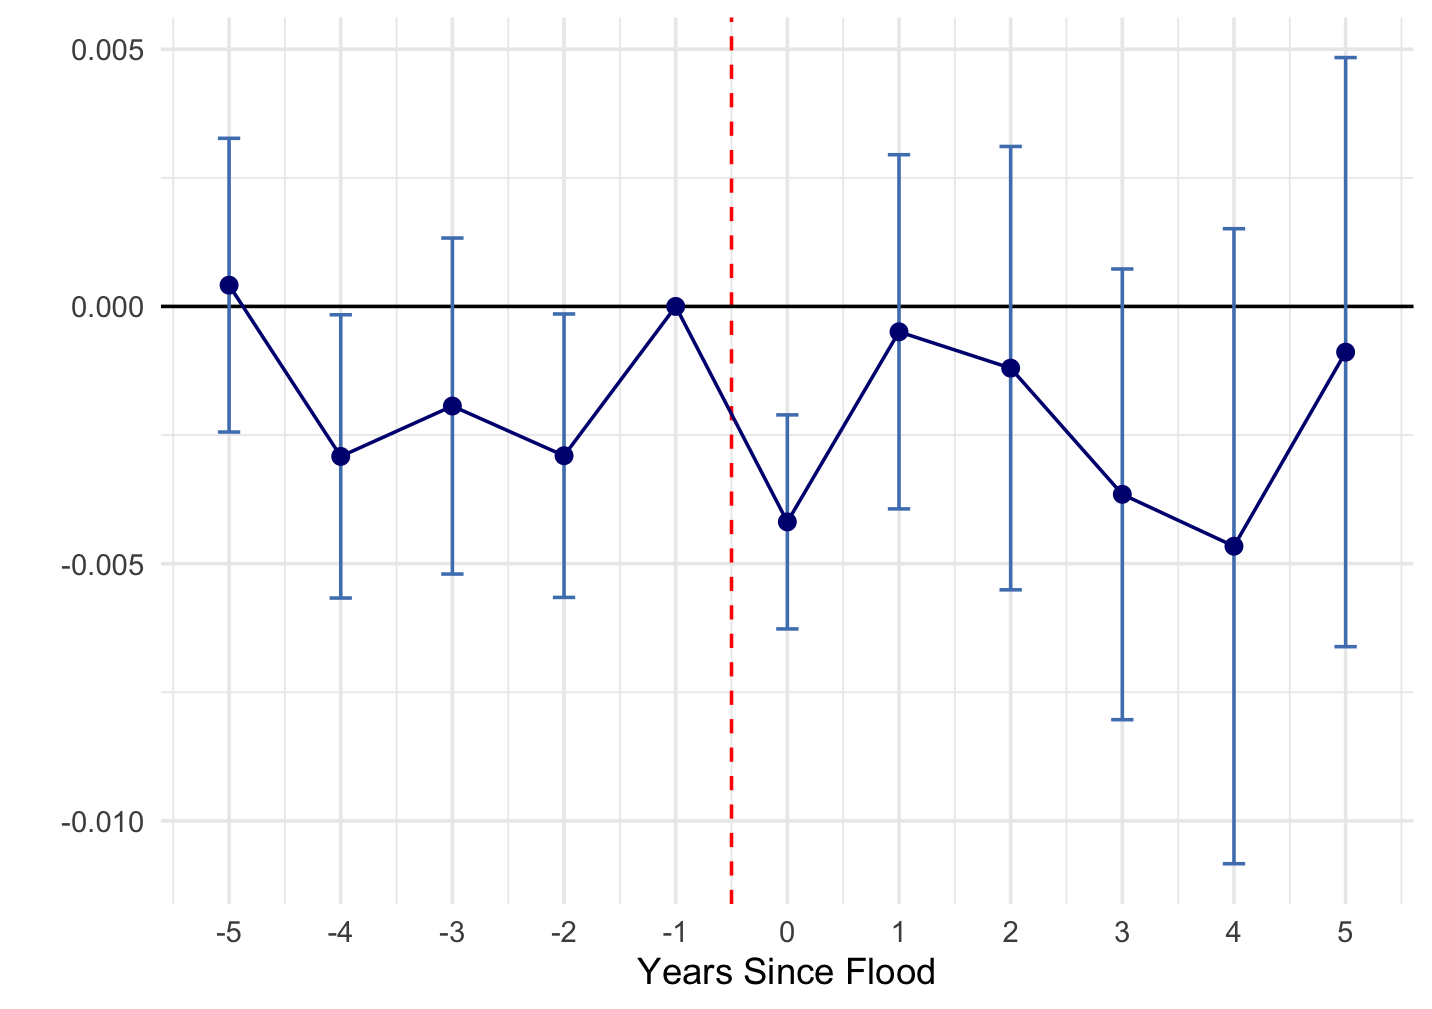
\includegraphics[width=\linewidth]{figures/Results/Analysis_Firms/share_CDD_weighted.png}
    \subcaption{\textbf{Share of temporary contracts}}
  \end{subfigure}
  \hfill
  \begin{subfigure}[t]{0.47\textwidth}
    \centering
    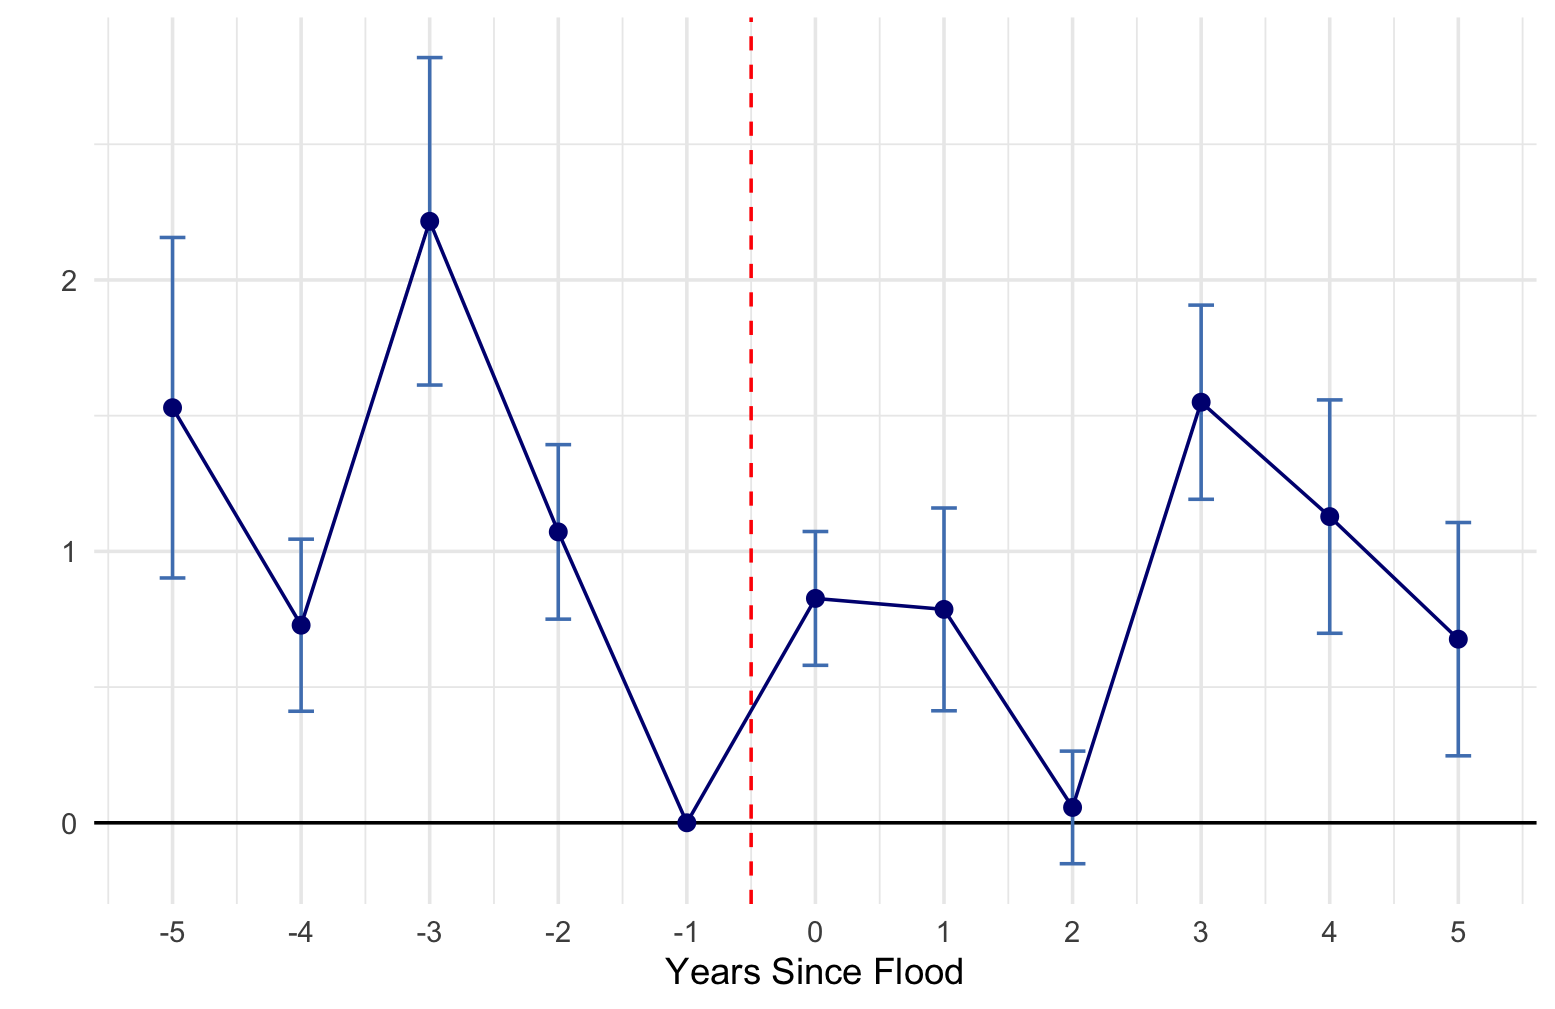
\includegraphics[width=\linewidth]{figures/Results/Analysis_Firms/ETP.png}
    \subcaption{\textbf{FTE Employment}}
  \end{subfigure}

  \vspace{0.8em}

  % Second row

  \begin{subfigure}[t]{0.47\textwidth}
    \centering
    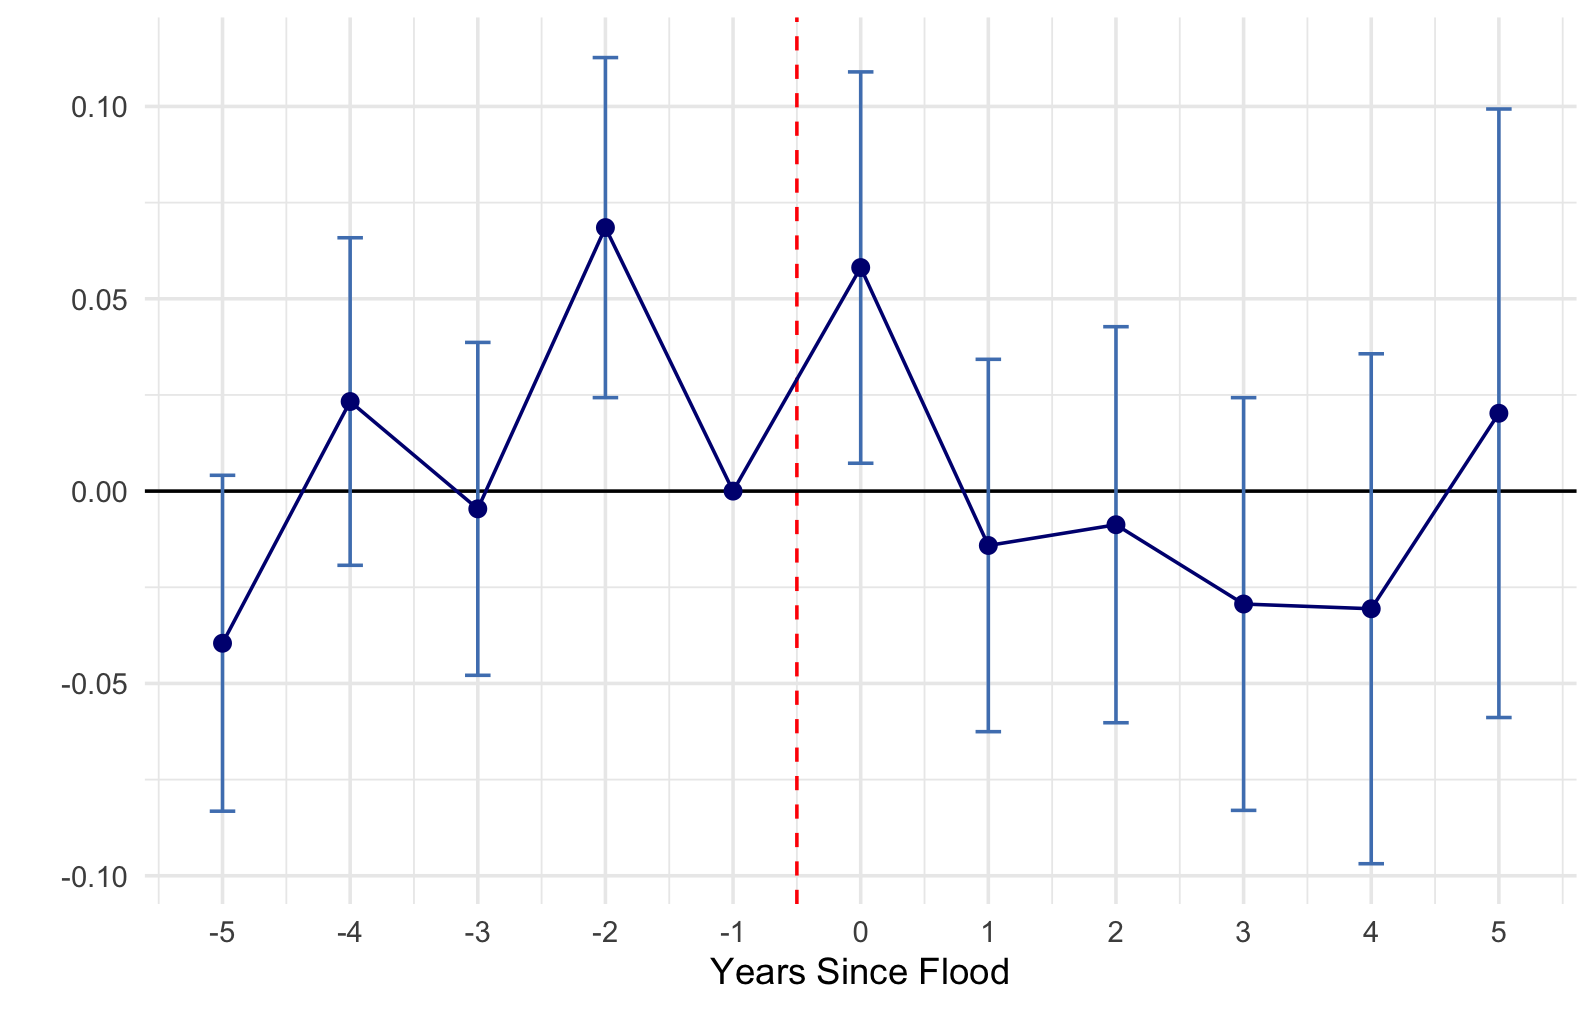
\includegraphics[width=\linewidth]{figures/Results/Analysis_Firms/HWAGE.png}
    \subcaption{\textbf{Hourly Wage}}
  \end{subfigure}
  \hfill
  \begin{subfigure}[t]{0.47\textwidth}
    \centering
    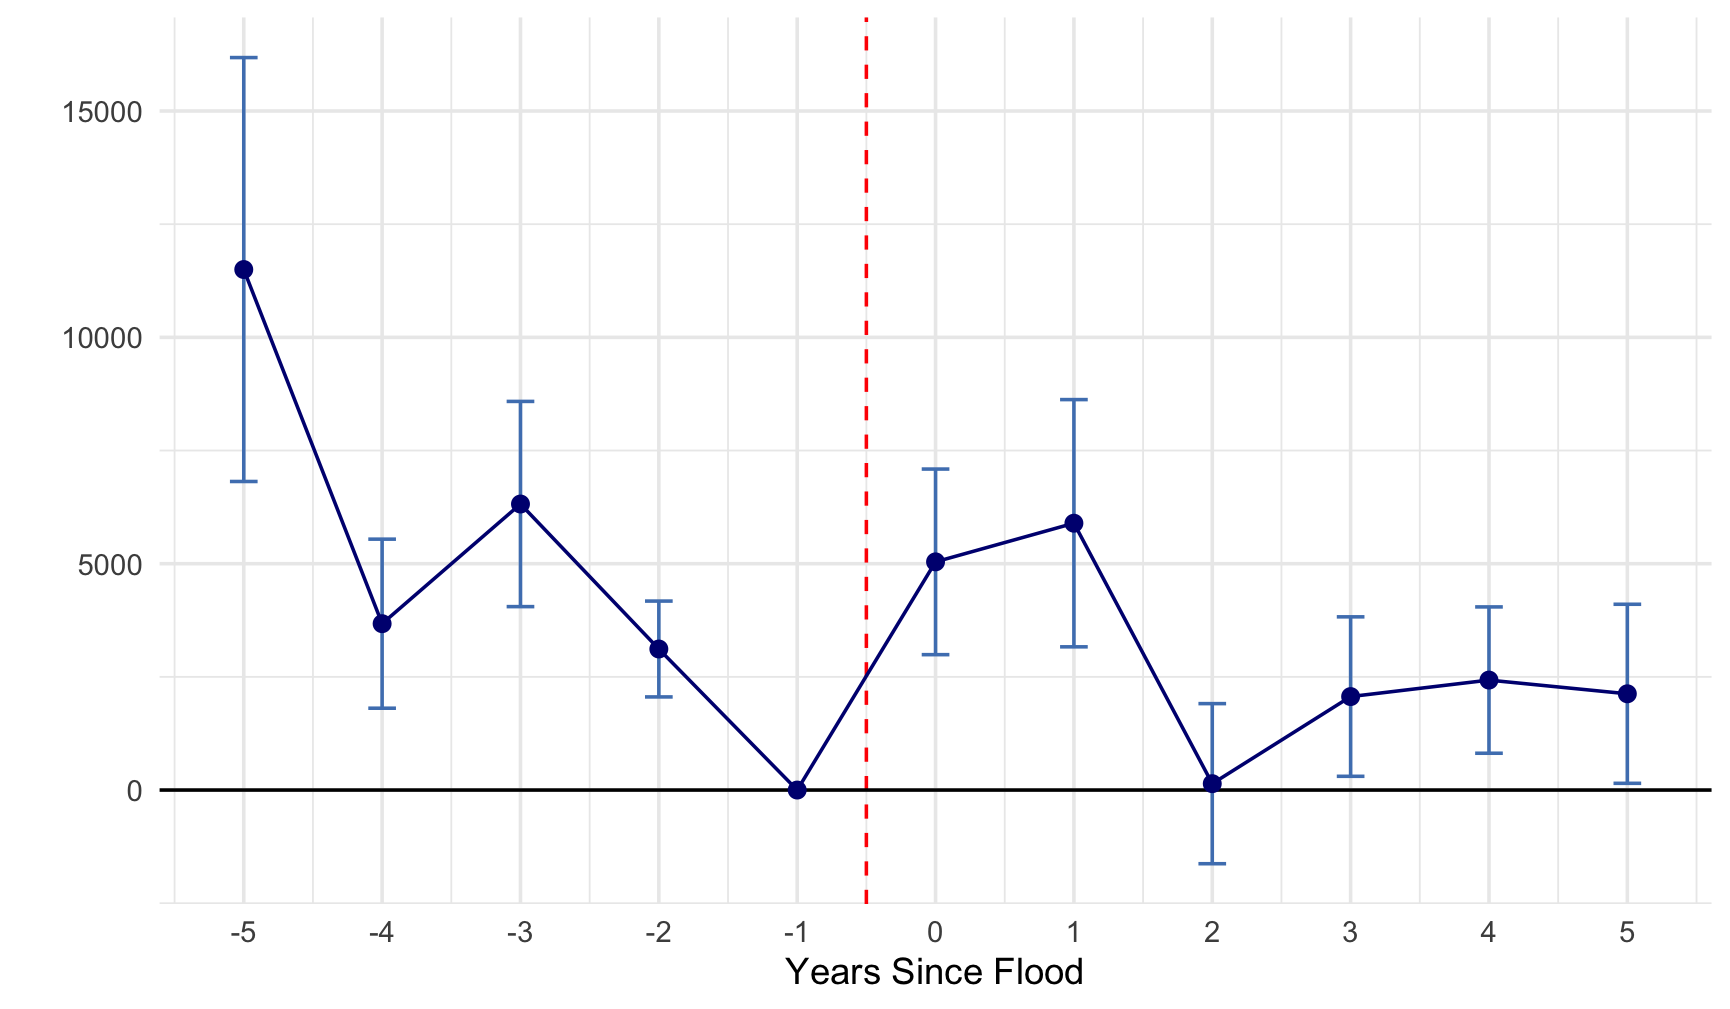
\includegraphics[width=\linewidth]{figures/Results/Analysis_Firms/HOURS.png}
    \subcaption{\textbf{Hours}}
  \end{subfigure}

    \vspace{0.8em}

  % Third row
\begin{subfigure}[t]{0.47\textwidth}
    \centering
    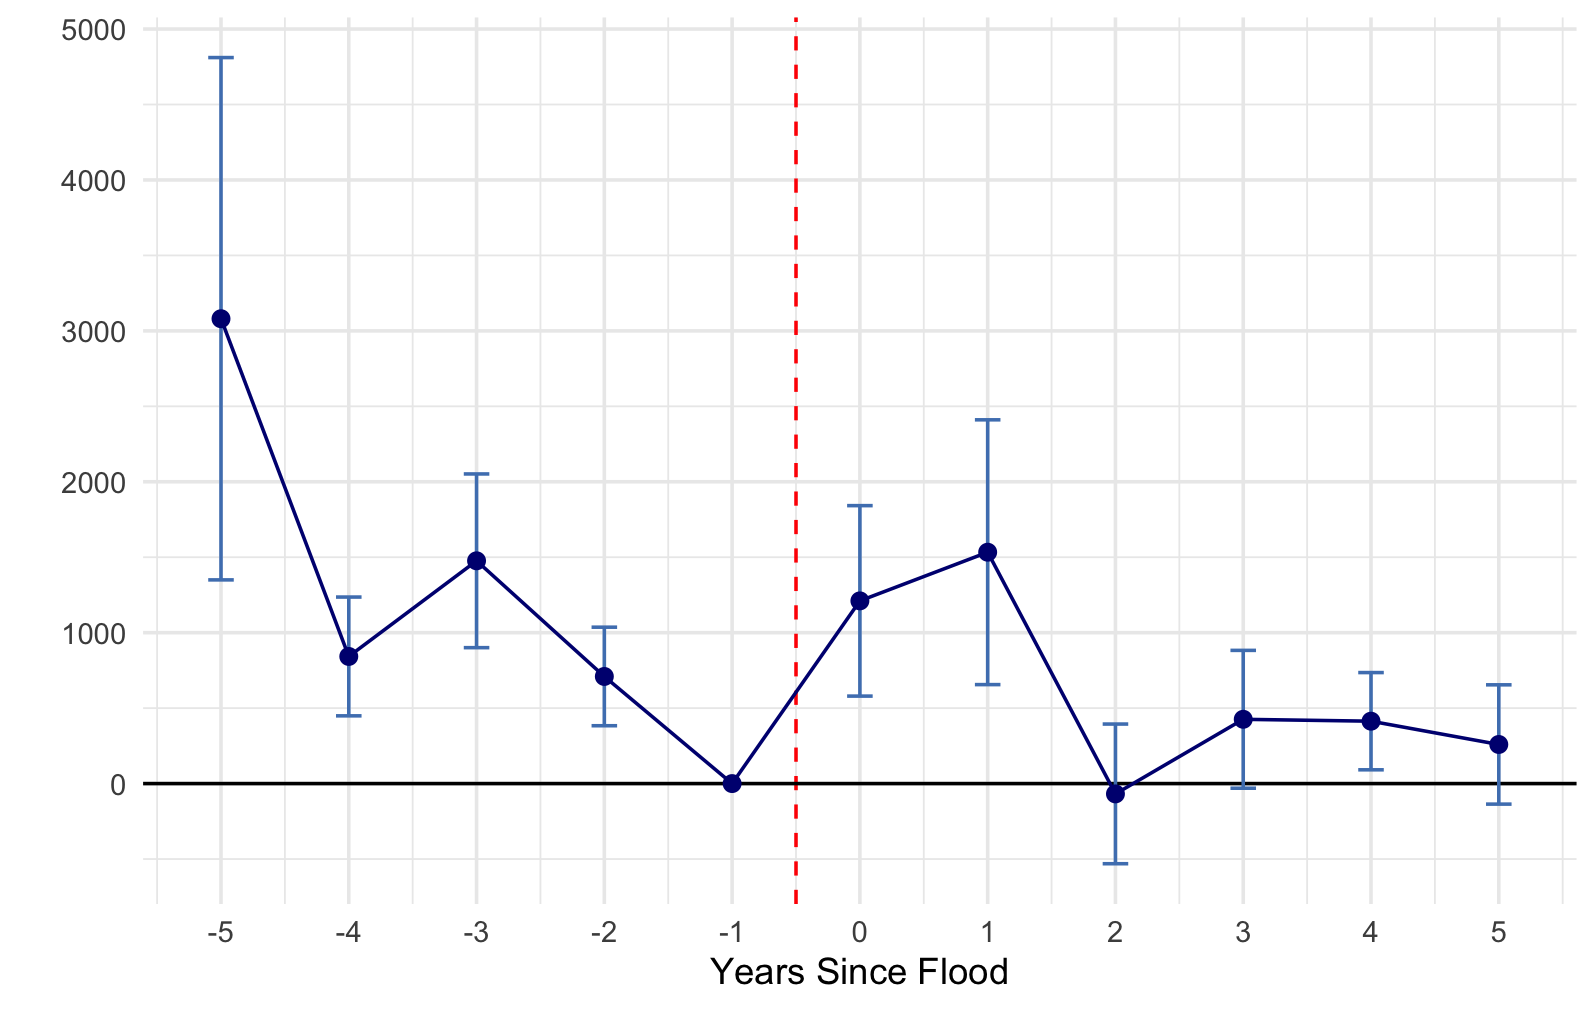
\includegraphics[width=\linewidth]{figures/Results/Analysis_Firms/redi_310_weighted.png}
    \subcaption{\textbf{Total Tunover (Revenue)}}
  \end{subfigure}
  \hfill
  \begin{subfigure}[t]{0.47\textwidth}
    \centering
    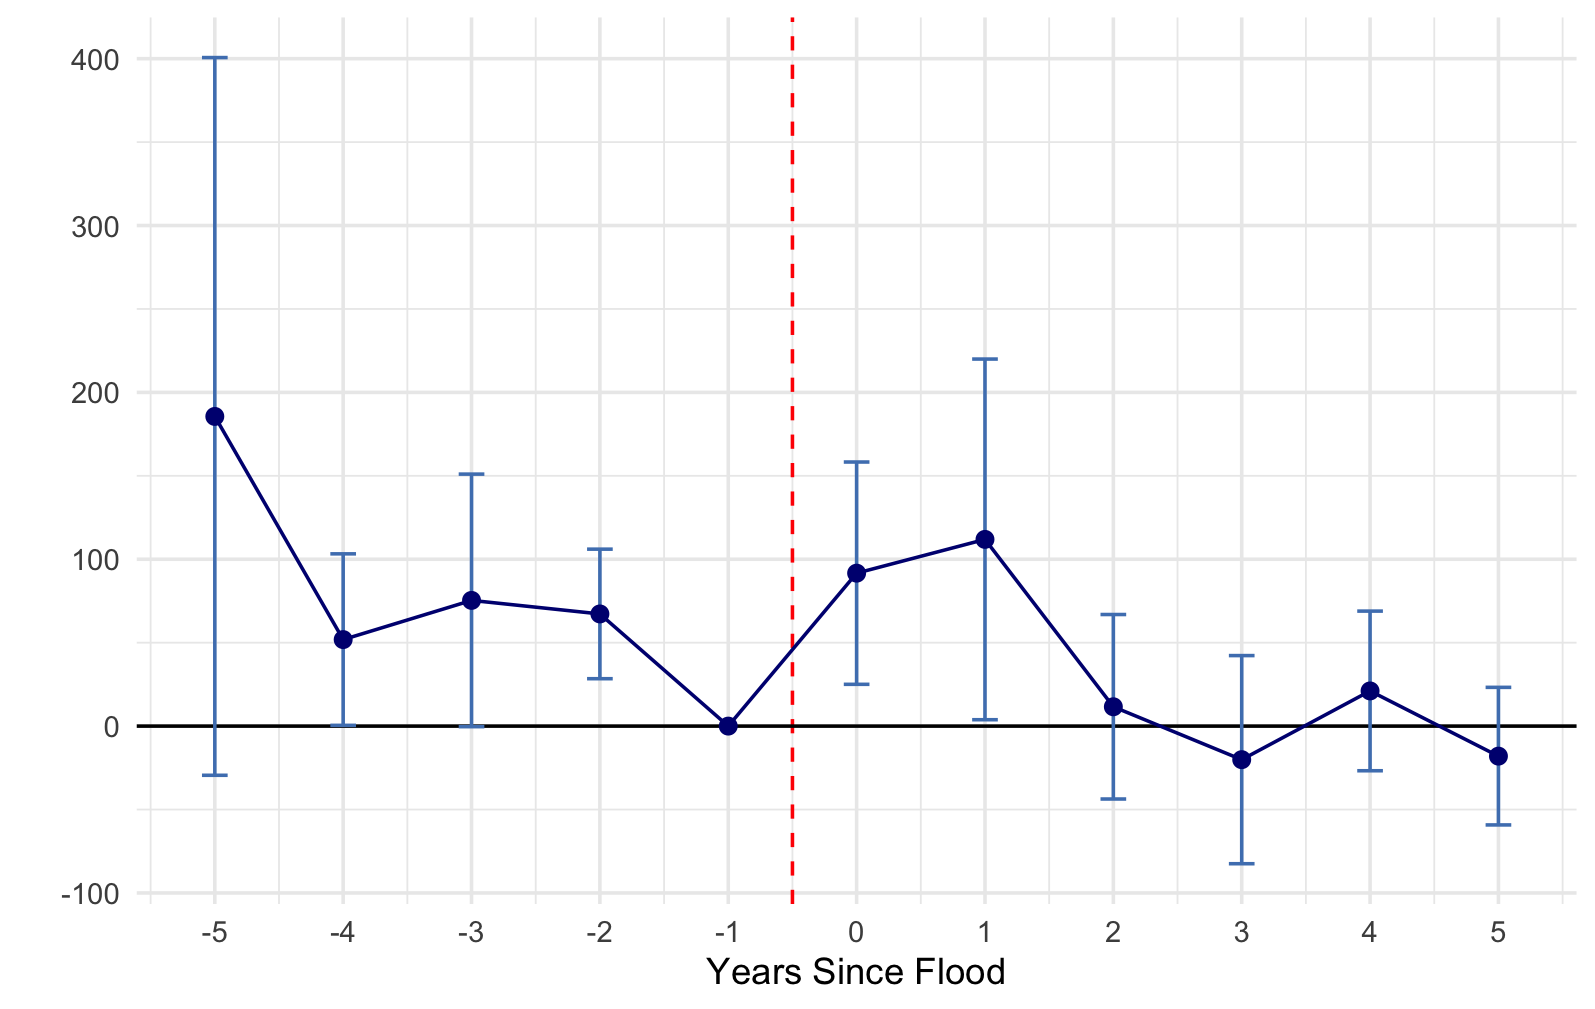
\includegraphics[width=\linewidth]{figures/Results/Analysis_Firms/319 profits.png}
    \subcaption{\textbf{Gross Profit before tax}}
  \end{subfigure}

\end{figure}



%%%%%%%%%%%%%%%%%%%%%%%%%%%%%%%%%%%%%%%%%%%%%%%%%%
%%%%%%%%%%%%%%%%%%%%%%%%%%%%%%%%%%%%%%%%%%%%%%%%%%
\clearpage
\section{Additional tables}
\label{sec:appendix_tables}
%%%%%%%%%%%%%%%%%%%%%%%%%%%%%%%%%%%%%%%%%%%%%%%%%%
%%%%%%%%%%%%%%%%%%%%%%%%%%%%%%%%%%%%%%%%%%%%%%%%%%



% Table - Flood Events count
\begin{table}[htbp]
  \centering
  \caption{\textbf{Table \ref{tab:flood_summary}:} History of flood events, affected communes and firms}
  \label{tab:flood_summary}
  \resizebox{\textwidth}{!}{%
  \begin{threeparttable}[b]
    \begin{tabular}{l r r r r r r r r}
      \toprule\toprule
      & \multicolumn{1}{c}{\textbf{CatNat decrees}} 
      & \multicolumn{1}{c}{\textbf{Communes affected}} 
      & \multicolumn{6}{c}{\textbf{Firms in sample}}\\[-0.2em]
      \cmidrule(lr){4-9}
      Year 
      & 
      & 
      & \multicolumn{3}{c}{Flooded}
      & \multicolumn{3}{c}{Total SIRETs} \\
      \cmidrule(lr){4-6} \cmidrule(lr){7-9}
      & & 
      & \multicolumn{1}{c}{$<$1 day} 
      & \multicolumn{1}{c}{1–22 days} 
      & \multicolumn{1}{c}{$>$22 days} 
      & \multicolumn{1}{c}{Affected} 
      & \multicolumn{1}{c}{Non-Affected} 
      & \multicolumn{1}{c}{Flood rate (\%)}\\
      \midrule
      2000 & 33 & 2\,227 & -- & -- & -- & -- & -- & -- \\
      2001 & 42 & 2\,879 & -- & -- & -- & -- & -- & -- \\
      2002 & 27 & 1\,163 & -- & -- & -- & -- & -- & -- \\
      2003 & 27 & 2\,261 & -- & -- & -- & -- & -- & -- \\
      2004 & 19 &   334 & -- & -- & -- & -- & -- & -- \\
      2005 & 21 &   842 & -- & -- & -- & -- & -- & -- \\
      2006 & 24 & 1\,072 & -- & -- & -- & -- & -- & -- \\
      2007 & 19 & 1\,070 & -- & -- & -- & -- & -- & -- \\
      2008 & 26 & 2\,177 & -- & -- & -- & -- & -- & -- \\
      2009 & 23 & 4\,425 & -- & -- & -- & -- & -- & -- \\
      2010 & 23 & 1\,981 & 24\,107 & 43\,415 & 0     & 67\,522 & 587\,707 & 10.31 \\
      2011 & 23 &   962 & 25\,834 & 35\,847 & 0     & 61\,681 & 669\,845 & 8.43 \\
      2012 & 18 &   729 & 16\,350 & 11\,930 & 21    & 28\,301 & 635\,386 & 4.26 \\
      2013 & 31 & 1\,511 & 29\,098 & 40\,948 & 145   & 70\,191 & 607\,992 & 10.35 \\
      2014 & 33 & 2\,057 & 26\,898 & 82\,310 & 129   & 109\,337 & 609\,840 & 15.20 \\
      2015 & 22 &   776 & 48\,124 & 12\,579 & 2     & 60\,705 & 629\,434 & 8.80 \\
      2016 & 29 & 2\,846 & 28\,609 & 61\,608 & 21    & 90\,238 & 546\,372 & 14.17 \\
      2017 & 23 &   303 & 15\,063 & 2\,017  & 0     & 17\,080 & 666\,863 & 2.50 \\
      2018 & 37 & 3\,426 & 76\,373 & 96\,275 & 753   & 173\,401 & 663\,240 & 20.73 \\
      2019 & 26 &   913 & 29\,246 & 63\,188 & 0     & 92\,434 & 728\,887 & 11.26 \\
      2020 & 28 & 1\,168 & -- & -- & -- & -- & -- & -- \\
      \bottomrule\bottomrule
    \end{tabular}
    \begin{tablenotes}[flushleft]
      \small
      \item \emph{Notes:} “Affected” firms are disaggregated by flood duration: less than 1 day (low), 1–22 days, and $>$22 days (high). The flood rate (\%) is the share of affected firms over the total observed firms in a given year.
    \end{tablenotes}
  \end{threeparttable}}
\end{table}



% Table: Flood counts 2000-2020
% \begin{table}[htbp]
  \centering
  \caption{\textbf{Table \ref{tab:flood_counts}}: Flood statistics (2000-2020)}
  \label{tab:flood_counts}
  \resizebox{0.8\textwidth}{!}{%
  \begin{threeparttable}[b]
    \begin{tabular}{lrrrrr}
      \toprule\toprule
      Total floods & SIRETs & $<$ 1 day & 1 to 22 days & $>$ 22 days & Avg. years between \\
      \midrule
      0 & 1\,884\,703 & -- & -- & -- & -- \\
      1 & 625\,619 & 285\,690 & 339\,106 & 823 & -- \\
      2 & 150\,801 & 145\,024 & 156\,381 & 197 & 3.69 \\
      3 & 45\,475 & 66\,798 & 69\,588 & 39 & 3.29 \\
      4 & 18\,178 & 33\,148 & 39\,555 & 9 & 2.74 \\
      5 & 7\,820 & 16\,941 & 22\,157 & 2 & 2.62 \\
      6 & 2\,423 & 5\,614 & 8\,923 & 1 & 2.41 \\
      7 & 723 & 1\,903 & 3\,158 & 0 & 2.08 \\
      8 & 189 & 562 & 950 & 0 & 1.95 \\
      9 & 81 & 183 & 546 & 0 & 1.74 \\
      \midrule
      Total & 2\,736\,012 & 555\,863 (20.32\%) & 640\,364 (23.41\%) & 1\,071 (0.04\%) & -- \\
      \bottomrule\bottomrule
    \end{tabular}%
    \begin{tablenotes}[flushleft]
      \small
      \item \emph{Notes:} Data aggregated from flood exposure at the SIRET level. Percentages in parentheses represent the proportion of SIRETs affected by each flood intensity relative to total SIRETs.
    \end{tablenotes}
  \end{threeparttable}%
  }
\end{table}


% Table: Flood counts 2010-2019
\vspace{1cm}
\begin{table}[htbp]
  \centering
  \caption{\textbf{Table \ref{tab:flood_counts19}}: Flood statistics (2010--2019)}
  \label{tab:flood_counts19}
  \resizebox{0.8\textwidth}{!}{%
  \begin{threeparttable}[b]
    \begin{tabular}{lrrrrr}
      \toprule\toprule
      Total floods & SIRETs & Low (1 day) & Medium (1–22 days) & High ($>$22 days) & Avg. years between \\
      \midrule
      0 & 1\,455\,888 & -- & -- & -- & -- \\
      1 & 445\,886 & 180\,317 & 264\,724 & 845 & -- \\
      2 & 95\,527 & 80\,767 & 110\,084 & 203 & 1.39 \\
      3 & 27\,988 & 37\,561 & 46\,380 & 23 & 1.34 \\
      4 & 9\,592 & 16\,628 & 21\,740 & 0 & 1.30 \\
      5 & 1\,799 & 3\,469 & 5\,526 & 0 & 1.28 \\
      6 & 422 & 929 & 1\,603 & 0 & 1.24 \\
      7 & 13 & 31 & 60 & 0 & 1.06 \\
      \midrule
      Total & 2\,037\,115 & -- & -- & -- & -- \\
      %Total & 2\,037\,115 & 239\,702 (11.8\%) & 449\,117 (22.0\%) & 1\,071 (0.05\%) & -- \\
      \bottomrule\bottomrule
    \end{tabular}
    \begin{tablenotes}[flushleft]
      \small
      \item \emph{Notes:} Flood counts refer to the number of floods experienced by a commune between 2010 and 2019. Low/Medium/High intensity is based on total duration of the CatNat decree.
    \end{tablenotes}
  \end{threeparttable}
  }
\end{table}

% Table: SIRET YEARS
\begin{table}[htbp]
  \centering
  \caption{\textbf{Table \ref{tab:n_years_firms}}: Number of Years Firms Appear in the Data (2010--2019)}
  \label{tab:n_years_firms}
  \resizebox{0.5\textwidth}{!}{%
    \begin{threeparttable}[b]
      \begin{tabular}{cccc}
        \toprule\toprule
        Years Present & Frequency & Percent & Cumulative \\
        \midrule
        1  & 600,750  & 8.81  & 8.81  \\
        2  & 840,246  & 12.32 & 21.13 \\
        3  & 842,433  & 12.35 & 33.48 \\
        4  & 829,720  & 12.16 & 45.64 \\
        5  & 720,665  & 10.57 & 56.21 \\
        6  & 694,524  & 10.18 & 66.39 \\
        7  & 513,807  & 7.53  & 73.92 \\
        8  & 511,576  & 7.50  & 81.42 \\
        9  & 364,680  & 5.35  & 86.77 \\
        10 & 902,460  & 13.23 & 100.00 \\
        \midrule
        Total & 6,820,861 & 100.00 & -- \\
        \bottomrule\bottomrule
      \end{tabular}
      \begin{tablenotes}[flushleft]
        \small
        \item \emph{Notes:} This table shows how many years (out of 10 between 2010 and 2019) each SIRET appears in the data. Approximately 13\% of firms are present for the full decade.
      \end{tablenotes}
    \end{threeparttable}
  }
\end{table}



% Table - LOnger results
%\begin{table}[!htbp]
\centering
\caption{\textbf{Table \ref{tab:lpdid_results}:} \textsc{OLD TABLE -- LP-DiD event-study estimates with bin-level observations}}
\label{tab:lpdid_results}

\resizebox{14.5cm}{!}{
\begin{tabular}{@{\extracolsep{6pt}}p{8cm}ccr}
\\[-1.8ex]\hline
\hline \\[-1.8ex]
& \multicolumn{2}{c}{\textit{Dependent variable:}} & \\
\cline{2-3}
\\[-1.8ex] & EFF\_3112 (Employment) & AVGWAGE\_3112 (Wages) & Obs (bin) \\
\hline \\[-1.8ex]
Event time $-5$ & $-$0.031 & $-$16.83 & 521,227 \\
                & (0.033)  & (48.47)  &         \\[0.15em]
Event time $-4$ & 0.027    & $-$40.41 & 650,620 \\
                & (0.027)  & (42.21)  &         \\[0.15em]
Event time $-3$ & 0.015    & $-$33.38 & 794,878 \\
                & (0.019)  & (37.73)  &         \\[0.15em]
Event time $-2$ & $-$0.004 & $-$45.89 & 989,096 \\
                & (0.016)  & (37.39)  &         \\[0.15em]
Event time $-1$ & 0 (reference) & 0 (reference) & -- \\ [0.15em]
Event time $0$  & $-$0.169$^{***}$ & $-$214.19$^{***}$ & 1,369,029 \\
                & (0.040)         & (30.07)            &            \\[0.15em]
Event time $1$  & $-$0.230$^{***}$ & $-$268.61$^{***}$ & 807,004 \\
                & (0.055)         & (49.05)            &         \\[0.15em]
Event time $2$  & $-$0.088$^{*}$   & $-$236.09$^{***}$ & 585,341 \\
                & (0.045)         & (62.64)            &         \\[0.15em]
Event time $3$  & $-$0.144$^{***}$ & $-$185.56$^{***}$ & 442,005 \\
                & (0.055)         & (65.99)            &         \\[0.15em]
Event time $4$  & $-$0.163$^{***}$ & $-$202.26$^{***}$ & 322,004 \\
                & (0.056)         & (69.77)            &         \\[0.15em]
Event time $5$  & $-$0.176$^{**}$  & $-$187.39$^{**}$  & 224,432 \\
                & (0.082)         & (80.31)            &         \\[0.35em]

\hline \\[-1.8ex]
Total observations     & 1,369,029 & 1,237,240 & -- \\
Mean per bin           & 676,977   & 608,899   & -- \\
\hline
\hline \\[-1.8ex]
\multicolumn{4}{p{17cm}}{\textit{Note:} Cluster-robust standard errors (at the INSEE\_COM level) in parentheses. $^{*}p<0.1$; $^{**}p<0.05$; $^{***}p<0.01$. Event time $-1$ is the omitted reference category.} \\[0.6em]

\multicolumn{4}{p{17cm}}{\texttt{lpdid(Y, unit = SIRET, time = ANNEE, treat = flood\_dummy\_extreme, pre\_window = 5, post\_window = 5, controls = c(floods\_last\_10y, floods\_last\_5y, floods\_last\_3y, years\_since\_last\_flood), cluster = INSEE\_COM, absorb = i.flood\_risk\_group\#i.Section\#\#c.ANNEE, weights = w\_att)}}
\end{tabular}}
\end{table}








%\subsection{Establishment-level data}


%\section{Robustness Checks}


\begin{landscape}
\scriptsize
\begin{ThreePartTable}
\begin{TableNotes}[flushleft]\footnotesize
%\item \textit{Note:} PCS-based variables are constructed by .
\end{TableNotes}

\begin{longtable}{@{}p{9cm}p{9cm}@{}}
\caption{\textbf{Table \ref{tab:codebook}:} Variable Codebook, FARE-FICUS and DADS}\label{tab:codebook}\\
\toprule
\textbf{Variable} & \textbf{Description} \\
\midrule
\endfirsthead
\multicolumn{2}{l}{\textbf{(Continued)}}\\
\toprule
\textbf{Variable} & \textbf{Description} \\
\midrule
\endhead

\bottomrule
\insertTableNotes
\endlastfoot

% --- FARE–FICUS ---
\multicolumn{2}{l}{\textit{FARE–FICUS dataset}}\\[0.2em]
\texttt{SIREN}            & Legal-unit identifier\\
\texttt{ANNEE}            & Calendar year\\
\texttt{depcom}           & Commune code (head office)\\
\texttt{ape\_diff}        & Main activity (NAF Rev. 1)\\
\texttt{r004}             & VAHT – IMPOTAX + SUBVEXP (value added)\\
\texttt{redi\_e001}       & Headcount on 31 Dec\\
\texttt{redi\_e200}       & Average salaried headcount (EFFSALM)\\
\texttt{redi\_r310}       & Total turnover (CATOTAL)\\
\texttt{redi\_r216}       & Wages and salaries (SALTRAI)\\
\texttt{b319}             & Current gross profit before tax (PBCAI)\\
\texttt{b330}             & Loans and related debts (EMPDETT)\\
\texttt{CAPISOC}          & Share capital\\
\texttt{VAHT}             & Value added excl. tax\\
\texttt{IMPOTAX}          & Taxes and duties\\
\texttt{SUBVEXP}          & Operating subsidies\\[0.5em]

% --- DADS ---
\multicolumn{2}{l}{\textit{DADS dataset}}\\[0.2em]
\texttt{YEAR}             & Calendar year\\
\texttt{SIREN}            & Legal-unit identifier\\
\texttt{SIRET}            & Establishment identifier\\
\texttt{ZEMPT}            & Employment-zone code\\
\texttt{Code\_commune}    & INSEE commune code (establishment)\\[0.5em]

% --- PCS aggregates ---
\multicolumn{2}{l}{\textit{PCS-based aggregates (available by socio-professional category)}}\\[0.2em]
\texttt{EFF\_ALL}         & Total salaried employment\\
\texttt{HOURS}            & Total hours worked\\
\texttt{HWAGE}            & Mean hourly wage\\
\texttt{AVGWAGE}          & Mean annual wage\\
\texttt{ETP}              & Full-time equivalents\\
\texttt{EFF\_3112}        & Headcount on 31 Dec (establishment level)\\ [0.5em]

% --- Employment dynamics ---
\multicolumn{2}{l}{\textit{Employment dynamics}}\\[0.2em]
\texttt{HIRES}            & Hires during year\\
\texttt{HIRES2}           & Alternative hires definition\\
\texttt{SEPARATIONS}      & Separations during year\\[0.5em]

% --- Contract shares ---
\multicolumn{2}{l}{\textit{Contract-type shares}}\\[0.2em]
\texttt{CDI}              & Share of open-ended contracts\\
\texttt{CDD}              & Share of fixed-term contracts\\
\texttt{interim}          & Share of temporary-agency contracts\\
\texttt{othercontract}    & Share of other contract types\\[0.5em]

% --- Short contracts ---
\multicolumn{2}{l}{\textit{Job spell by duration}}\\[0.2em]
\texttt{SHORTJOB\_1M}     & $\leq$ 1 month\\
\texttt{SHORTJOB\_3M}     & $\leq$ 3 months\\
\texttt{SHORTJOB\_6M}     & $\leq$ 6 months\\
\texttt{SHORTJOB\_LTO3M}  & $<$ 3 months\\
\texttt{SHORTJOB\_3TO6M}  & 3–6 months\\
\texttt{SHORTJOB\_6TO12M} & 6–12 months\\
\texttt{SHORTJOB\_MORE6M} & $>$ 6 months\\
\texttt{SHORTJOB\_MORE1Y} & $>$ 1 year\\

\end{longtable}
\end{ThreePartTable}
\end{landscape}
